\chapter{Week 4 -- Battery testing}
% As a general rule, do not put math, special symbols or citations
% in the abstract or keywords.
\section{Abstract}
This report presents the results of simple battery testing procedure required by the assignment\footnote{accesiable via \vomihwassignment}. Constant current charging and discharging pulses were applied to the cell under test in order to estimate basic parameters of the equivalent circuit model using the measured voltages. This procedure was repeated twice, once "manually" using a programmable power supply and DC load and once by programming a dedicated battery tester.

\section{Charging pulse}

During the charging experiment, the cell was charged by a constant current of 1 A for 20 seconds. Afterwards the cell was allowed to rest for 5 minutes to restore open circuit voltage. Charging was performed using the 
laboratory power supply \textit{BK PRECISION 9205}. No dedicated voltage measurement was provided, instead
only readings from the instrument's display with resolution of 1 mV were recorded. Readings inherently contain
voltage drop across the leads as well. Furthermore it is impossible to correctly record fast transients when enabling/disabling the power supply.
This significantly reduced the reliability of equivalent circuit parameters $R_0$, $R_1$ and $C_1$ estimated in section \ref{sec:4-params}.
The voltage profile together with the applied current is shown in Fig. \ref{fig:4-charging}.

\begin{figure}[htbp]
    \centering
    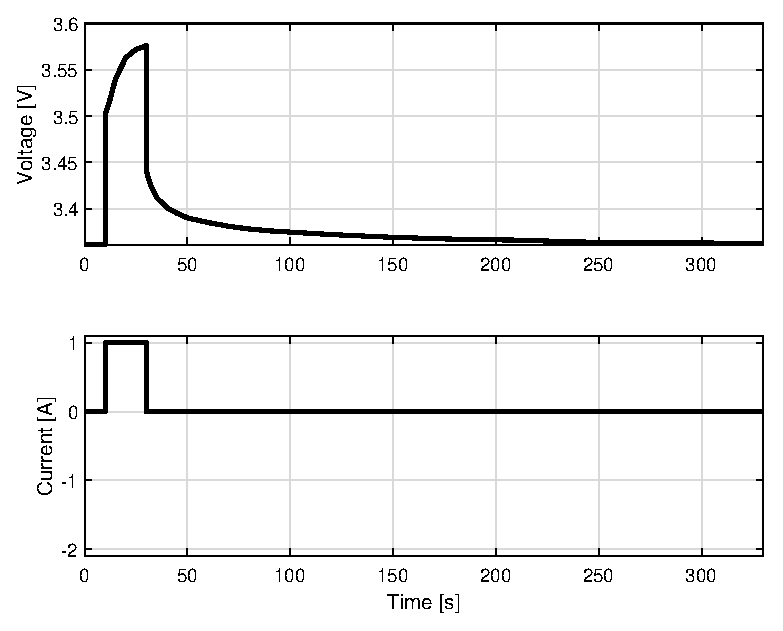
\includegraphics{figures/4/charge.eps}
    \caption{Voltage profile during the charging pulse experiment}
    \label{fig:4-charging}
\end{figure}

\section{Discharging pulse}
In this experiment, the cell was discharged by a constant current of 2 A for 20 seconds and allowed to rest for 5 minutes afterwards.
Discharging was performed using the DC programmable load \textit{BK PRECISION 8601}. Since no dedicated voltage measurement was provided, measurements from this experiment suffer from the same errors as discussed for the charging experiment. Measurements were recorded using the instrument's display with resolution of 0.1 mV.
The voltage profile together with the applied current is shown in Fig. \ref{fig:4-discharging}.


\begin{figure}[htbp]
    \centering
    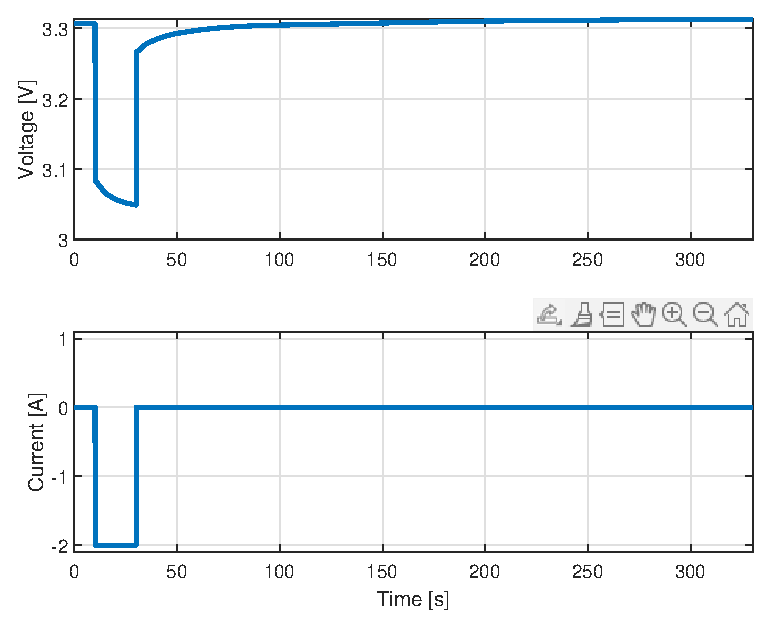
\includegraphics{figures/4/discharge.eps}
    \caption{Voltage profile during the discharging pulse experiment}
    \label{fig:4-discharging}
\end{figure}

\section{Automated experiment}
An automated battery tester \textit{Newell BT-4008Tn-5V12A-S1} was programmed to perform a complete experiment containing 20 seconds of (dis)charging interleaved by relaxation time. Since the instrument (and the experimental setup overall) is professional, it can be assumed that some lead resistance is compensated in the recorded data. The instrument was configured to save quantities with sampling period 100 ms to correctly record fast transients when applying new value of current. The voltage profile together with the applied current is shown in Fig. \ref{fig:4-automated}.

\begin{figure}[htbp]
    \centering
    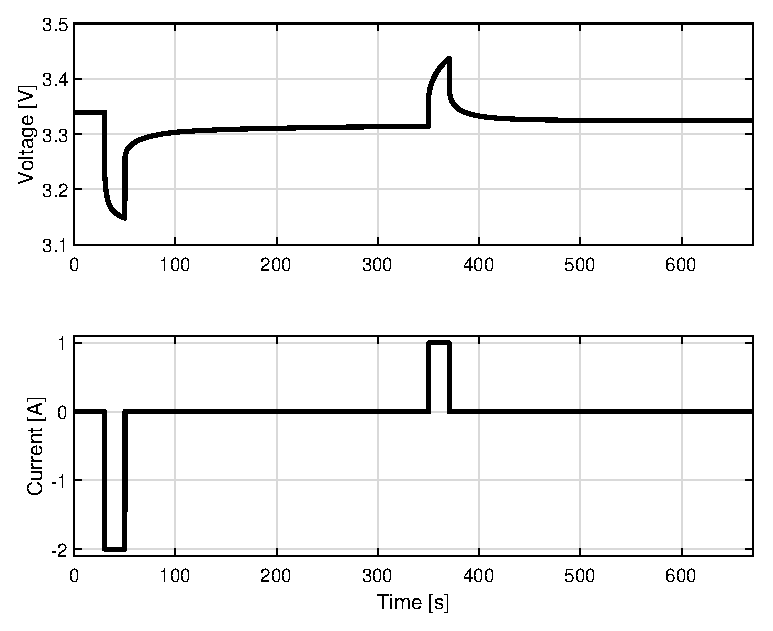
\includegraphics{figures/4/automated.eps}
    \caption{Voltage profile during the automated experiment}
    \label{fig:4-automated}
\end{figure}

\section{Parameter estimation}
\label{sec:4-params}
Data recorded during three experiments were used to estimate parameters of the equivalent circuit model with series impedance $R_0$ and one RC element $R_1$, $C_1$. Estimated values are shown in table \ref{tab:4-params}. It can be concluded that although the experimental setup for manual charging/discharging was very simple, it yielded reasonable estimates that are at least within the order of magnitude from the expected value. Automated measurements performed by the programmable battery tester are far more accurate. This manifests especially in the case of parameter $R_0$, whose value is almost equal for both automated discharge as well as charge experiment. It is not possible to give a certain estimate of $R_0$
for either of the manual experiments due to low refresh rate of instruments' displays. Recording a video of instrument's screen also isn't a particularly error resistant and high sampling rate method for data processing.

\begin{table}[htbp]
    \centering
    \begin{tabular}{c|c|c|c}
         Experiment& $R_0$ [$\Omega$] & $R_1$ [$\Omega$] & $C_1$ [F] \\\hline
         Manual discharge  & 1.116e-01  &   2.355e-02  &   2.547e+03 \\
         Manual charge & 1.410e-01   &  7.801e-02 &    7.6897e+02 \\
         Automated discharge & 5.664e-02  &   2.825e-02  &   2.124e+03 \\
         Automated charge & 5.701e-02   &  5.539e-02  &   1.083e+03
  
    \end{tabular}
    \caption{Estimated parameters of the cell model}
    \label{tab:4-params}
\end{table}
